%%%%%%%%%%%%%%%%%%%%%%%%%%%%%%%%%% NAME %%%%%%%%%%%%%%%%%%%%%%%%%%%%%
%%%%%%%%%%%%%%%%%
\section{Complementary Filter}
%%%%%%%%%%%%%%%%%

%%%%%%%%%%%%%%%%
\subsection{Gyroscope}
\begin{frame}{Complementary Filter}{Gyroscope}
A gyroscope measures angular velocity by integrating small intervals to find the orientations.
\begin{figure}
	\centering
	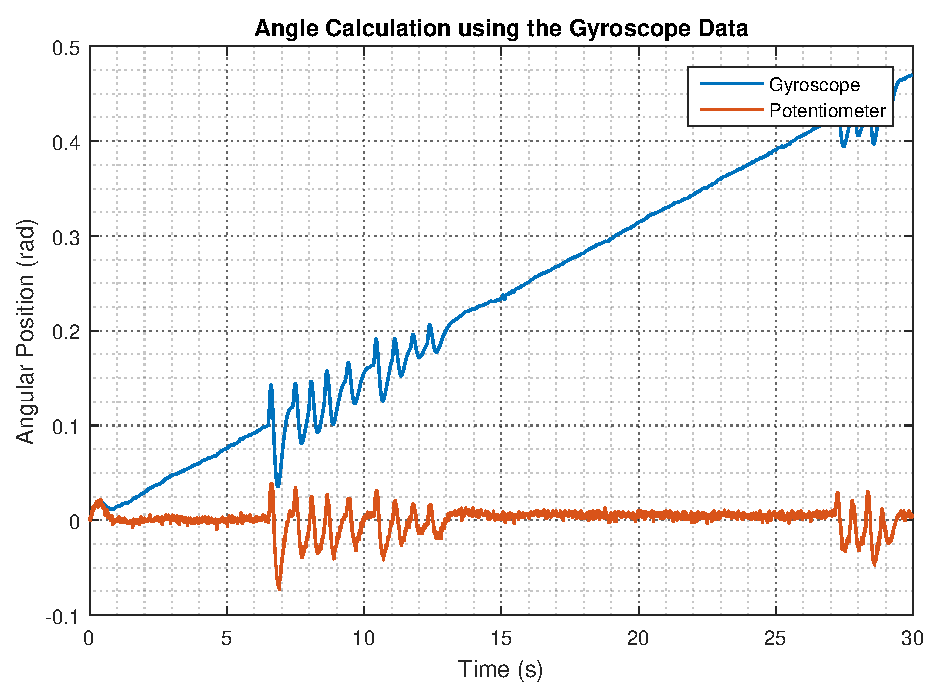
\includegraphics[scale=0.4]{Pictures/angleGyro.pdf}
\end{figure}

The problems with the gyroscope are:
	\begin{itemize}
		\item {By integrating, the error is accumulating over time.}
		\item {The gyroscope may experiencing drifting errors from small and slow movement.}
	\end{itemize}
\end{frame}
%%%%%%%%%%%%%%%
%%%%%%%%%%%%%%%%
\subsection{Accelerometers}
\begin{frame}{Complementary Filter}{Accelerometers}
An accelerometer measures inertial force, such as gravity and relies on a constant gravitational pull with respect to the Earth, and the calculations orientation can be found.
\begin{figure}
	\centering
	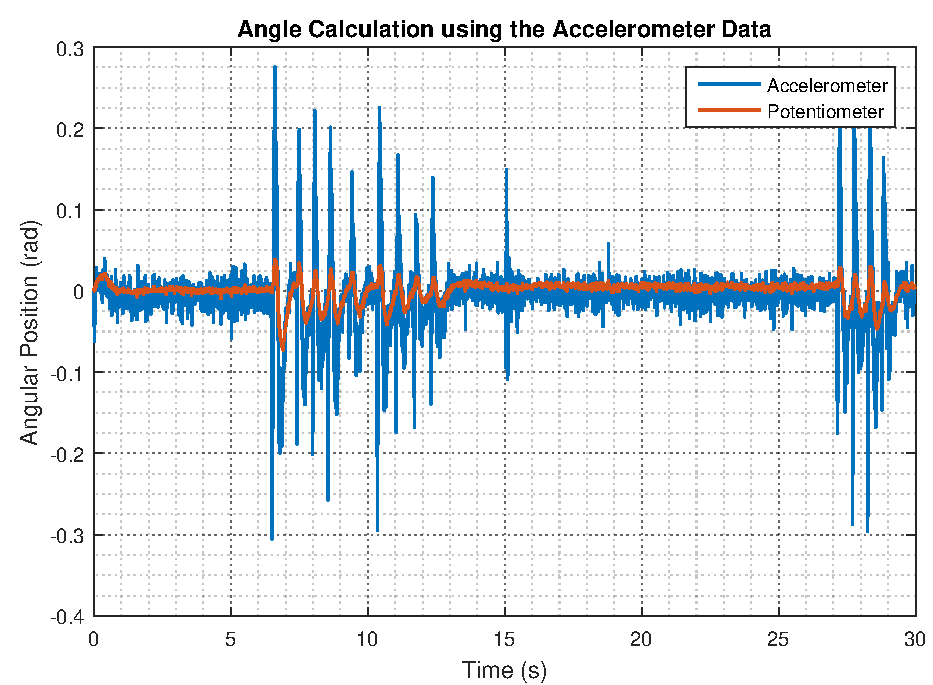
\includegraphics[scale=0.4]{Pictures/angleAcc.pdf}
\end{figure}

The problems for accelerometers are:
\begin{itemize}
	\item {They are very sensitive to mechanical noise and vibrations.}
\end{itemize}
\end{frame}
%%%%%%%%%%%%%%%%
%%%%%%%%%%%%%%%%
\subsection{Sensor Fusion}
\begin{frame}{Complementary Filter}{Sensor Fusion}
Data from accelerometers and gyroscopes can be combined for a better estimate of orientation than using only accelerometer data.\linebreak

The combined data can help fix noise and drift error. A method is to use a complementary filter.
\begin{figure}
	\centering
	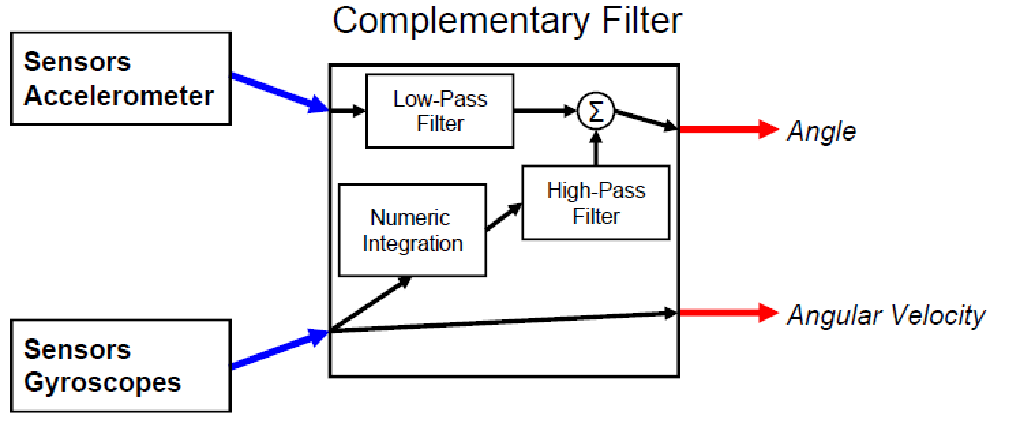
\includegraphics[scale=0.5]{Pictures/Complementary.pdf}
\end{figure}
Complementary filter advantages is:
\begin{itemize}
	\item {Fast estimates of angle and much less lag than low-pass filter alone.}
	\item {Not very processor-intensive.}
\end{itemize}
\end{frame}
%%%%%%%%%%%%%%%%
%%%%%%%%%%%%%%%%
\subsection{Cut-off Frequency}
\begin{frame}{Complementary Filter}{Cut-off Frequency}
High pass and low pass filters with the same cut-off frequency. 
\begin{figure}
	\centering
	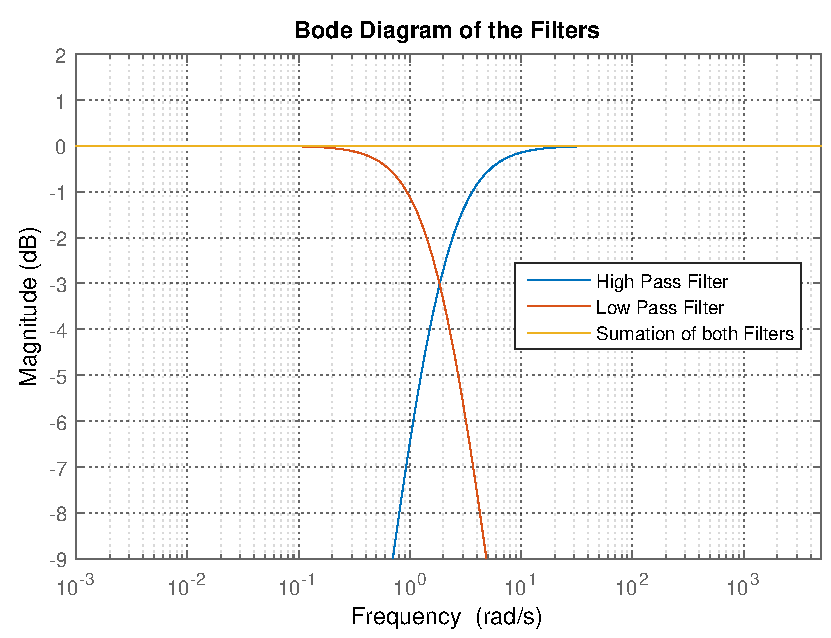
\includegraphics[scale=0.5]{Pictures/bodeFilters.pdf}
\end{figure}
The summation of both cut-off frequency gives a gain of 1.
\end{frame}
%%%%%%%%%%%%%%%%
%%%%%%%%%%%%%%%%
\subsection{Compare Results}
\begin{frame}{Complementary Filter}{Compare Results}
The complementary filter compared with the data from the potentiometer.
	\begin{figure}
		\centering
		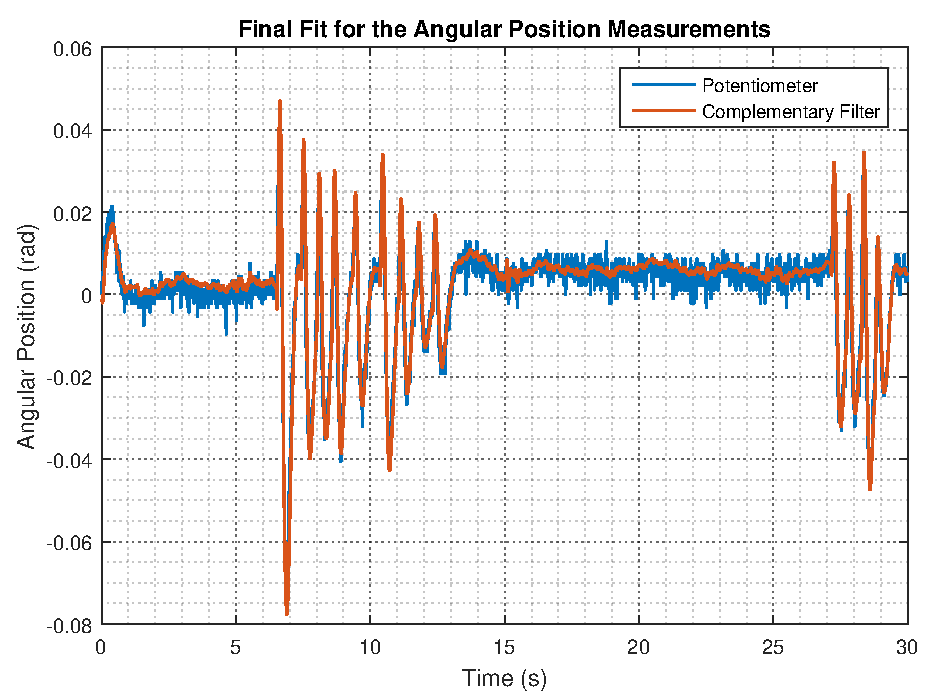
\includegraphics[scale=0.5]{Pictures/filterSensTool.pdf}
	\end{figure}
The two measurements match closely.
\end{frame}
%%%%%%%%%%%%%%%%
%%%%%%%%%%%%%%%%%%%%%%%%%%%%%%%%%% NAME %%%%%%%%%%%%%%%%%%%%%%%%%%%%%
%%%%%%%%%%%%%%%%
\section{Acceptance Test}
%%%%%%%%%%%%%%%%

%%%%%%%%%%%%%%%%
\subsection{Requirements Test}

\begin{frame}{Acceptance Test}{Requirements Test}
- The Cubli should be able to balance starting from an unstable equilibrium position and null velocity.\linebreak

\begin{minipage}{\linewidth}
	\begin{minipage}{0.45\linewidth}
		\begin{figure}[H]
			\centering
			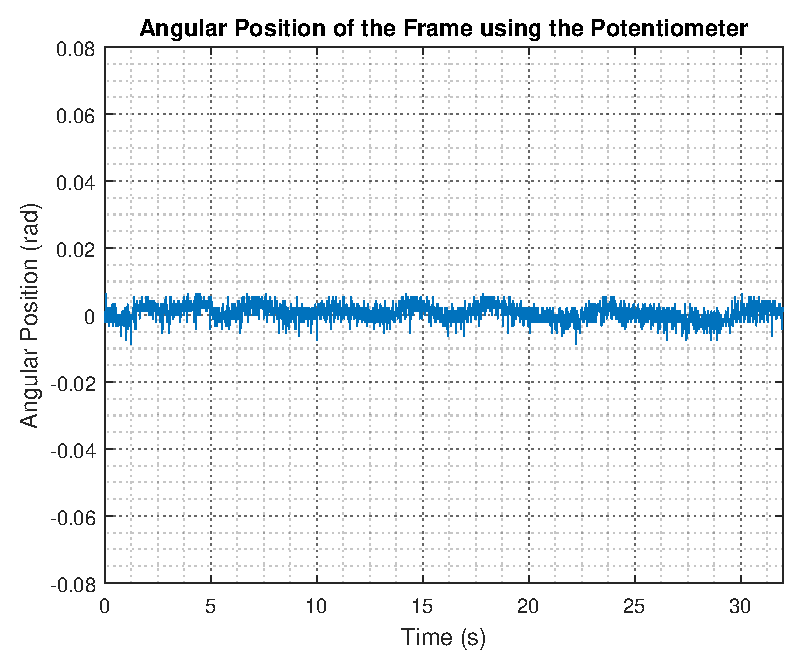
\includegraphics[scale=.345]{Pictures/testReq1}
		\end{figure}
	\end{minipage}
	\hspace{0.03\linewidth}
	\begin{minipage}{0.45\linewidth}
		\begin{figure}[H]\vspace{0mm}
			\centering
			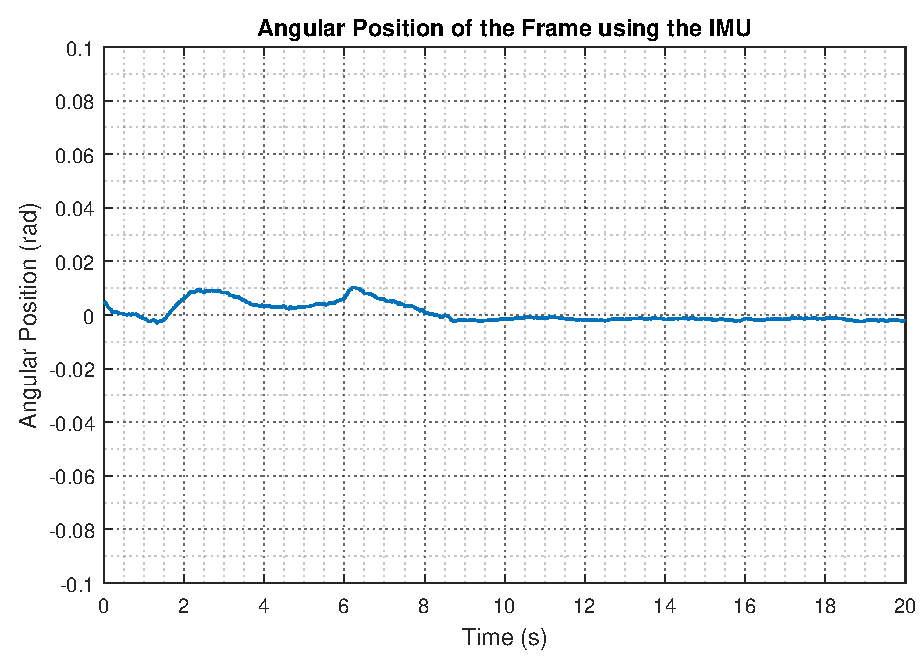
\includegraphics[scale=.345]{Pictures/testReq1_IMU}
		\end{figure}
	\end{minipage}
\end{minipage}\linebreak

Angular position of the frame, when starting from equilibrium position.
	\begin{itemize}
		\item {Measured with the potentiometer.}
		\item {Calculated with the complementary filter.}
	\end{itemize}
	 
 
\end{frame}
%%%%%%%%%%%%%%%%
%%%%%%%%%%%%%%%%
\subsection{Requirements Test}

\begin{frame}{Acceptance Test}{Requirements Test}
- The prototype should be able to balance around 0 rad, even though the angle of inclination of the baseplate is changed within a reasonable range, using internally mounted sensors.
	
\begin{figure}
	\centering
	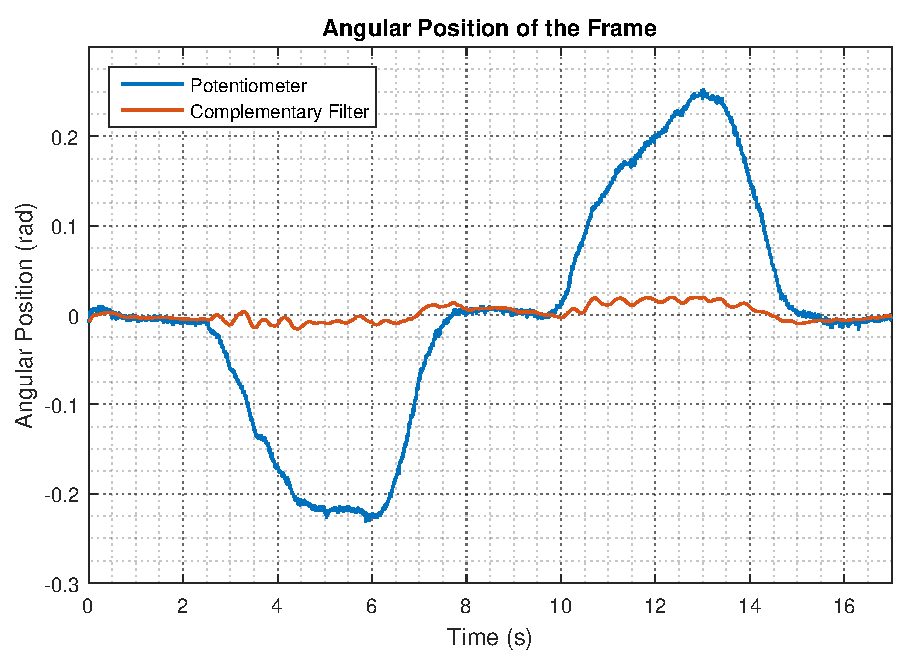
\includegraphics[scale=0.40]{Pictures/testReq2.pdf}
\end{figure}
Position of the frame which does not depend on the angle of the baseplate.
\end{frame}
%%%%%%%%%%%%%%%%

%%%%%%%%%%%%%%%%%%%%%%%%%%%%%%%%%%% NAME %%%%%%%%%%%%%%%%%%%%%%%%%%%%%
%%%%%%%%%%%%%%%%
\section{Conclusion}
%%%%%%%%%%%%%%%%

%%%%%%%%%%%%%%%%
\subsection{Conclusion}

\begin{frame}{Conclusion}{Cubli}
Maximum recovery angle while disturbances is applied:
	\begin{itemize}
		\item {The controller is capable of recovering from \si{0,08\ rad} (\si{4,58^\circ}).}
		\item {The controller is not able to recover from greater angle due to overshoot.}\linebreak
	\end{itemize}
	
Maximum catching angle with no initial velocity of the wheel is \si{0,2024\ rad} (\si{11,59^\circ}):
	\begin{itemize}
		\item {The controller is capable of catching the frame when it starts from \SI{-0,17}{rad}  (\si{-9,74^\circ}).}
		\item {The controller is not able to recover from greater angle due to overshoot.}\linebreak
	\end{itemize}
It is not possible to catch and balance the system in equilibrium position from a  greater angle than \SI{-0,17}{rad}  (\si{-9,74^\circ}).\linebreak
\end{frame}
%%%%%%%%%%%%%%%%
%%%%%%%%%%%%%%%%
\subsection{Conclusion}

\begin{frame}{Conclusion}{Cubli}
	Improving the system:
	\begin{itemize}
		\item {Measurements of the IMU could be improved by moving the sensor.}
		\item {Fusing Sensor data from IMU using a different filter type.}\linebreak
	\end{itemize}
	
It was also a requirement to be able to:
	\begin{itemize}
		\item {Keep it in upright position.}
		\item {Change the angle of the baseplate.}\linebreak
	\end{itemize}
	
In conclusion:
	\begin{itemize}
		\item {The state space controller constructed has been tested successfully within the requirements.}
	\end{itemize}
\end{frame}
%%%%%%%%%%%%%%%%